\documentclass{paper}
\usepackage[utf8]{inputenc}

\title{Projeto de Desenvolvimento}
\author{Joao Marcos Lyra Vieira }
\date{October 2019}

\usepackage{natbib}
\usepackage{graphicx}
\usepackage[a4paper, total={6in, 8in}]{geometry}

\begin{document}

\maketitle

\section{Introdução}
A disciplina Projeto de Desenvolvimento é ofertada aos alunos de ciência da computação(5º período), de Engenharia da computação(8º período) e e Design e tem como objetivo final a realização de um projeto que englobe todo o conhecimento já adquirido no curso, tais como conhecimentos técnicos como de empreendedorismo. Essa cadeira é considerada de suma importância pois representa ``um marco do fim do ciclo básico''.\citep{siteDaDisciplina}

\begin{figure}[h!]
\centering
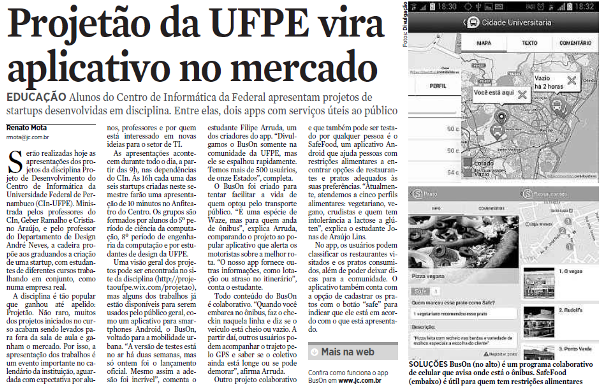
\includegraphics[scale=0.9]{jornal.png}
\caption{Manchete sobre a disciplina no Jornal do Comercio}
\label{fig:manchete}
\citep{ufpe}
\end{figure}

\section{Relevância}
O projeto realizado na matéria tem como um de suas exigências a criação de uma Startup e isso faz com que os alunos tenham uma visão mais real dos problemas enfrentados por empresas e ao mesmo tempo que produzem um projeto acadêmico eles produzem um projeto profissional que pode ser levado para fora da universidade como foi o caso da In Loco Media, que teve sua ideação um pouco antes do "Projetão"(como é chamada a disciplina pelo estudantes), mas só foi praticamente inicializada durante essa cadeira, atualmente, com quase 10 anos de mercado, a In Loco Media é uma das maiores empresas de tecnologia do Brasil. A relevância dessa matéria pode ser explicitada na frase dirigida a In Loco: ``um projeto de faculdade se tornou uma tecnologia de impacto global''.\citep{ArtigoLais}

\begin{figure}[h!]
\centering

\includegraphics[scale=0.4]{EmpresasDoProjetao.PNG}
\caption{Algumas das empresas que foram oriundas do Projeto de Desenvolvimento}
\label{EmpresasDoProjetao}
\citep{sitProjetao}
\end{figure}

\section{Relação com outras disciplinas}
A matéria tem como objetivo principal utilizar todos os conhecimentos adquiridos até o momento para a realização de um projeto que retorna um produto final pronto para entrar no mercado.Porém alguns conceitos da área de empreendedorismo são mais bem vistos na cadeira, tais como:``Gestão de Equipes Multidisciplinares, Gestão de Projetos, Identificação de Oportunidades para Inovação, Desenvolvimento e Validação de Produtos e Serviços, Comunicação em Inovação e Novos Negócios''\citep{sitProjetao} . Na teoria o "Projetão" é uma matéria que "finaliza" o curso, pois após o quinto período os estudantes não cursam mais cadeiras obrigatórias, somente as eletivas, que não tem menos importância, mas são escolhidas pelos próprios discentes e tendem a ser algo mais confortável para o mesmo.

\bibliographystyle{plain}
\bibliography{jmlv}
\end{document}
